%%%%%%%%%%%%%%%%%%%%%%%%%%%%%%%%%%%%%
%                                   %
% Compile with XeLaTeX and biber    %
%                                   %
% Questions or comments:            %
%                                   %
% joshua dot mcneill at uga dot edu %
%                                   %
%%%%%%%%%%%%%%%%%%%%%%%%%%%%%%%%%%%%%

\documentclass{beamer}
  % Read in standard preamble (cosmetic stuff)
  %%%%%%%%%%%%%%%%%%%%%%%%%%%%%%%%%%%%%%%%%%%%%%%%%%%%%%%%%%%%%%%%
% This is a standard preamble used in for all slide documents. %
% It basically contains cosmetic settings.                     %
%                                                              %
% Joshua McNeill                                               %
% joshua dot mcneill at uga dot edu                            %
%%%%%%%%%%%%%%%%%%%%%%%%%%%%%%%%%%%%%%%%%%%%%%%%%%%%%%%%%%%%%%%%

% Beamer settings
% \usetheme{Berkeley}
\usetheme{CambridgeUS}
% \usecolortheme{dove}
% \usecolortheme{rose}
\usecolortheme{seagull}
\usefonttheme{professionalfonts}
\usefonttheme{serif}
\setbeamertemplate{bibliography item}{}

% Packages and settings
\usepackage{fontspec}
  \setmainfont{Charis SIL}
\usepackage{hyperref}
  \hypersetup{colorlinks=true,
              allcolors=blue}
\usepackage{graphicx}
  \graphicspath{{../../figures/}}
\usepackage[normalem]{ulem}
\usepackage{enumerate}

% Document information
\author{M. McNeill}
\title[FREN2001]{Français 2001}
\institute{\url{joshua.mcneill@uga.edu}}
\date{}

%% Custom commands
% Lexical items
\newcommand{\lexi}[1]{\textit{#1}}
% Gloss
\newcommand{\gloss}[1]{`#1'}
\newcommand{\tinygloss}[1]{{\tiny`#1'}}
% Orthographic representations
\newcommand{\orth}[1]{$\langle$#1$\rangle$}
% Utterances (pragmatics)
\newcommand{\uttr}[1]{`#1'}
% Sentences (pragmatics)
\newcommand{\sent}[1]{\textit{#1}}
% Base dir for definitions
\newcommand{\defs}{../definitions}


  % Packages and settings

  % Document information
  \subtitle[Présentons-nous]{Présentons-nous}

  %% Custom commands
  % Subsection/frame titles

\begin{document}
  % Read in the standard intro slides (title page and table of contents)
  \begin{frame}
    \titlepage
    \tiny{Office: % Basically a variable for office hours location
Gilbert 121\\
          Office hours: % Basically a variable for office hours
 lundi, mercredi, vendredi 10:10--11:10
}
  \end{frame}

  \begin{frame}{Revue}
    \begin{center}
      \begin{tabular}{l | l l | l l}
  \multicolumn{5}{c}{être \gloss{to be}} \\
      & \multicolumn{2}{l |}{singulier} & \multicolumn{2}{l}{pluriel} \\
  \hline
  1re & je         & suis             & nous        & sommes \\
  2e  & tu         & es               & vous        & êtes \\
  \hline
  3e  & il (masc)  &                  & ils (masc)  & \\
      & elle (fem) & est              & elles (fem) & sont \\
      & on         &                  &             & \\
\end{tabular}

    \end{center}
  \end{frame}

  \begin{frame}{Revue}
    \begin{center}
      \begin{tabular}{l l l l}
        \multicolumn{4}{c}{Les pronoms disjoints} \\
        \hline
        \alert{moi}  & je   & \alert{nous}  & nous / on \\
        \alert{toi}  & tu   & \alert{vous}  & vous \\
        \alert{lui}  & il   & \alert{eux}   & ils \\
        \alert{elle} & elle & \alert{elles} & elles \\
      \end{tabular}
    \end{center}
    \begin{itemize}
      \item \sout{c'est je} $\to$ c'est \alert{moi}
      \item \sout{c'est eux} $\to$ \alert{ce sont} eux
    \end{itemize}
  \end{frame}

  \begin{frame}{Qui est-ce? \gloss{Who is that?}}
    \gloss{Say who that is and confirm with a \lexi{pronom disjoint}.}
    \centering
    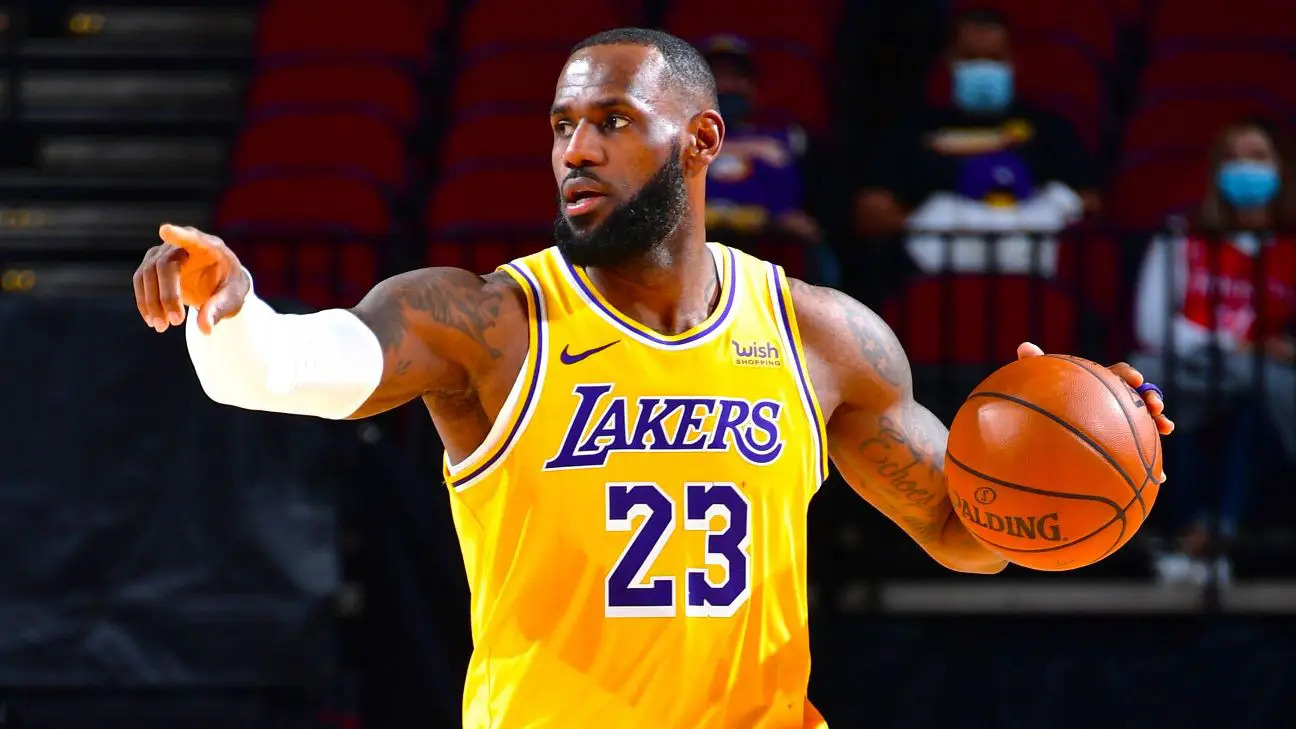
\includegraphics[scale=0.2]{lebron.jpg}

    \uncover<2->{
      C'est \alert<3->{LeBron James}.
    }

    \uncover<3->{
      C'est \alert{lui}.
    }
  \end{frame}

  \begin{frame}{Qui est-ce? \gloss{Who is that?}}
    \centering
    
\includegraphics[scale=0.22]{hulk_et_she-hulk.jpg}

    \uncover<2->{
      Ce sont \alert<3->{Hulk et She-Hulk}.
    }

    \uncover<3->{
      Ce sont \alert{eux}.
    }
  \end{frame}

  \begin{frame}{Qui est-ce? \gloss{Who is that?}}
    \centering
    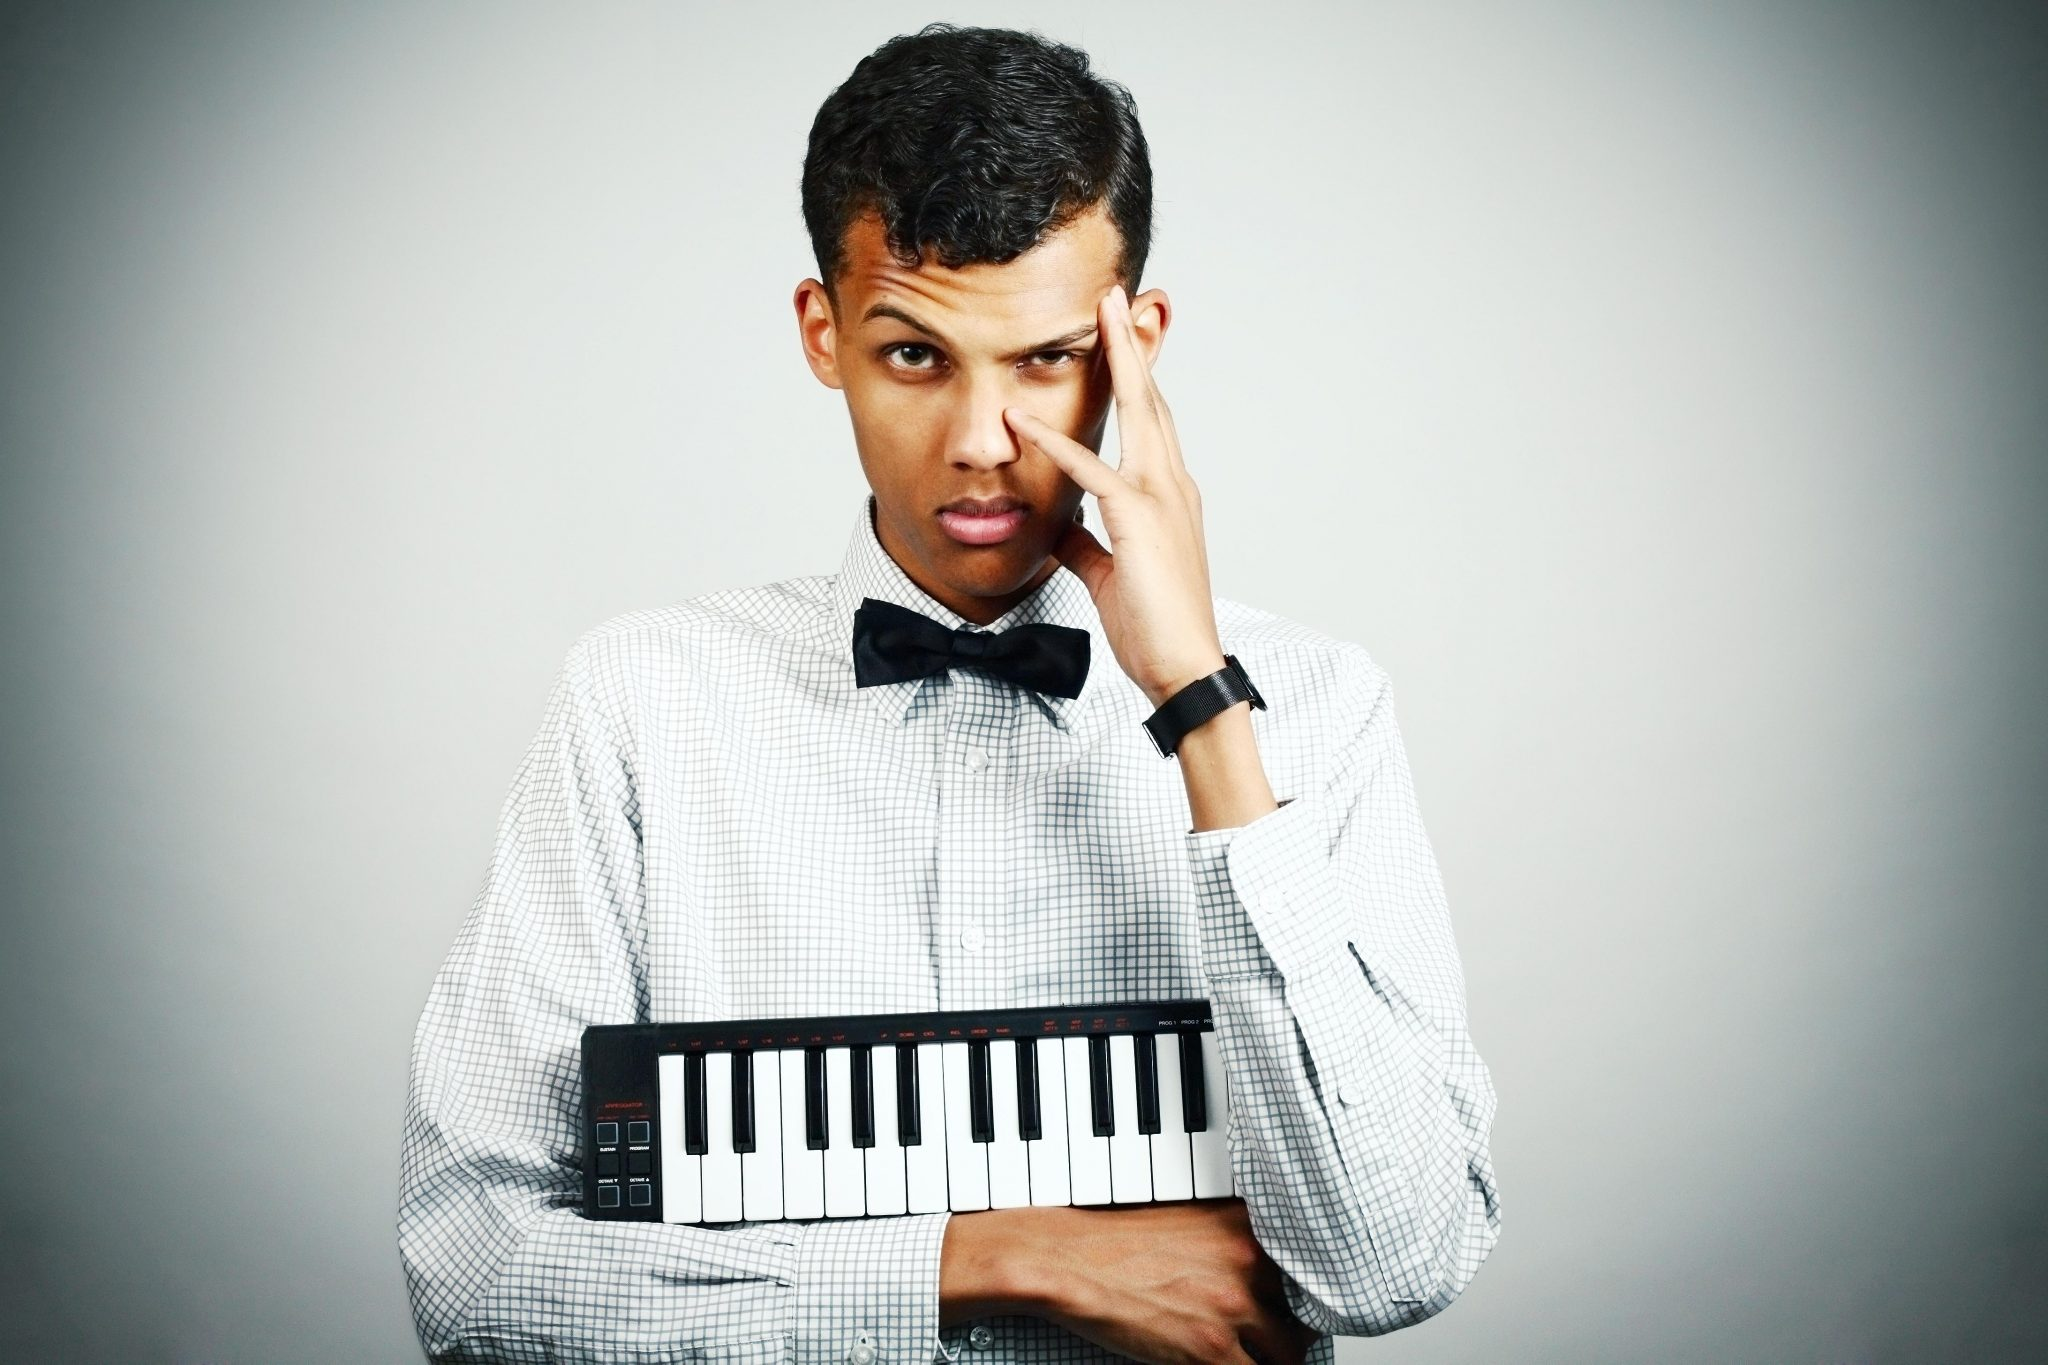
\includegraphics[scale=0.15]{stromae.jpg}

    \uncover<2->{
      C'est \alert<3->{Stromae}.
    }

    \uncover<3->{
      C'est \alert{lui}.
    }
  \end{frame}

  \begin{frame}{Qui est-ce? \gloss{Who is that?}}
    \centering
    
\includegraphics[scale=0.35]{margaret_cho.jpg}

    \uncover<2->{
      C'est \alert<3->{Margaret Cho}.
    }

    \uncover<3->{
      C'est \alert{elle}.
    }
  \end{frame}

  \begin{frame}{Qui est-ce? \gloss{Who is that?}}
    \centering
    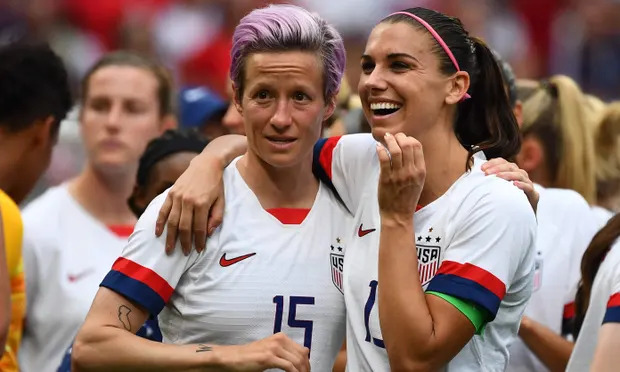
\includegraphics[scale=0.4]{rapinoe_et_morgan.jpg}

    \uncover<2->{
      Ce sont \alert<3->{Megan Rapinoe et Alex Morgan}.
    }

    \uncover<3->{
      Ce sont \alert{elles}.
    }
  \end{frame}

  \begin{frame}{Qui est-ce? \gloss{Who is that?}}
    \centering
    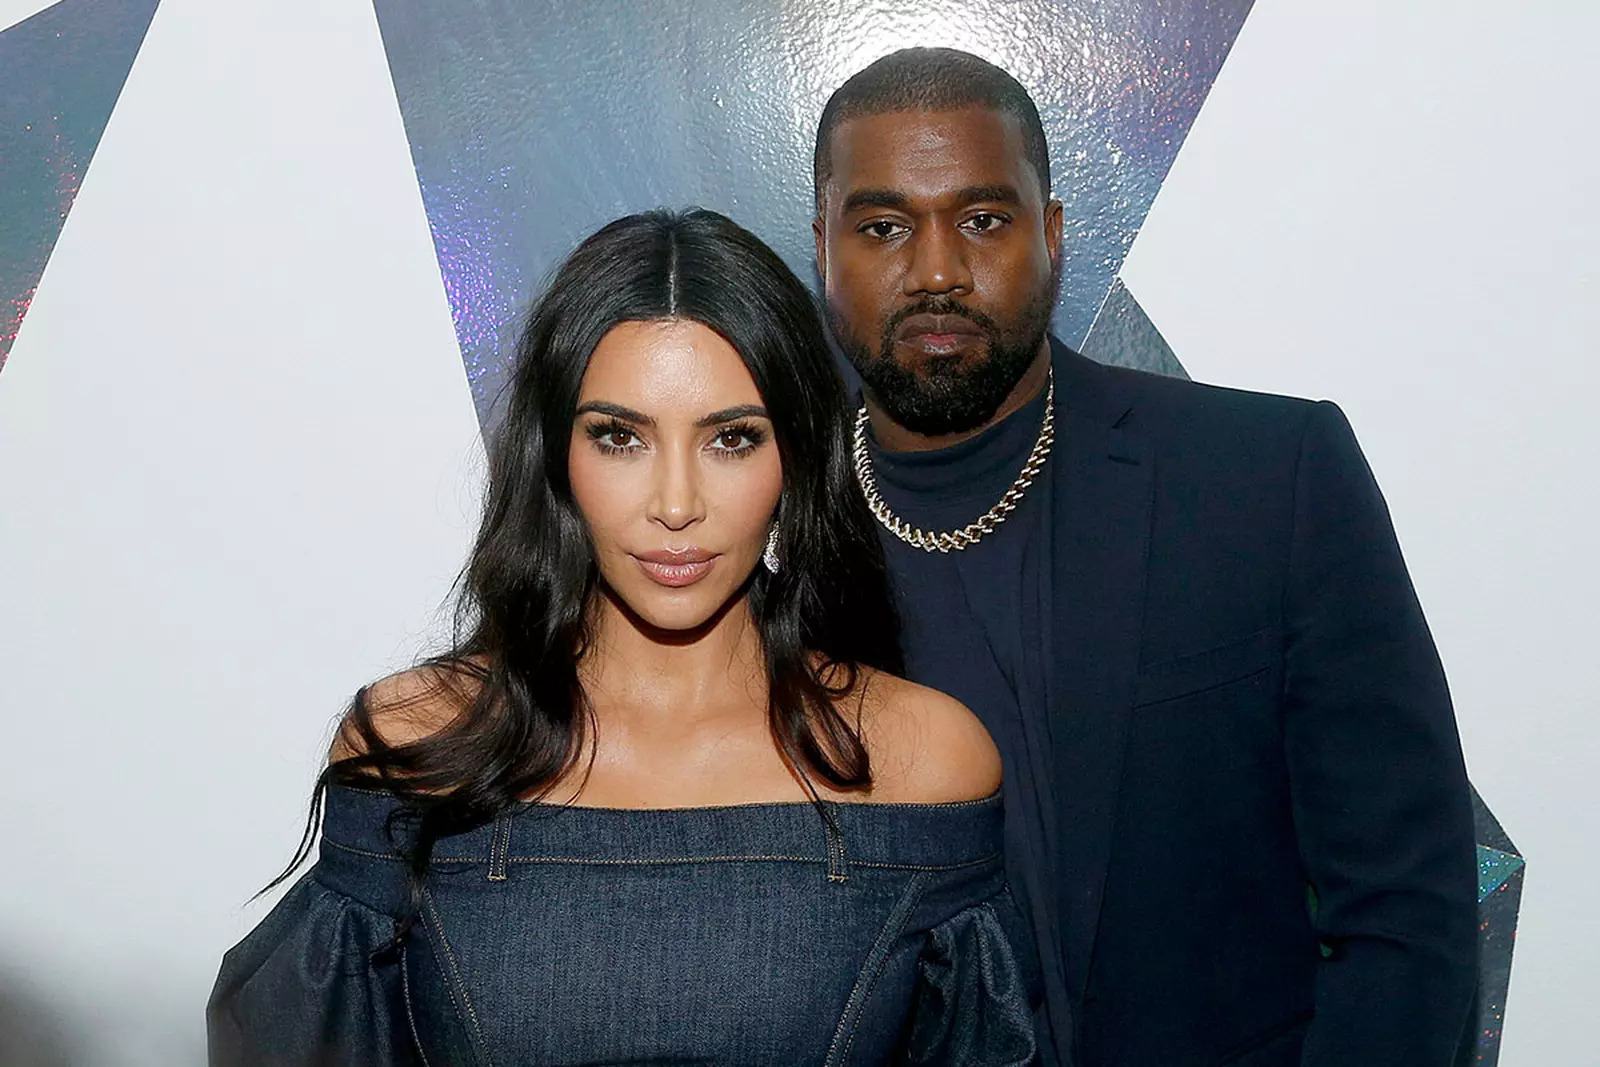
\includegraphics[scale=0.15]{kanye_et_kim.jpg}

    \uncover<2->{
      Ce sont \alert<3->{Kim Kardashian et Kanye West}.
    }

    \uncover<3->{
      Ce sont \alert{eux}.
    }
  \end{frame}

  \begin{frame}{Qui est-ce? \gloss{Who is that?}}
    \centering
    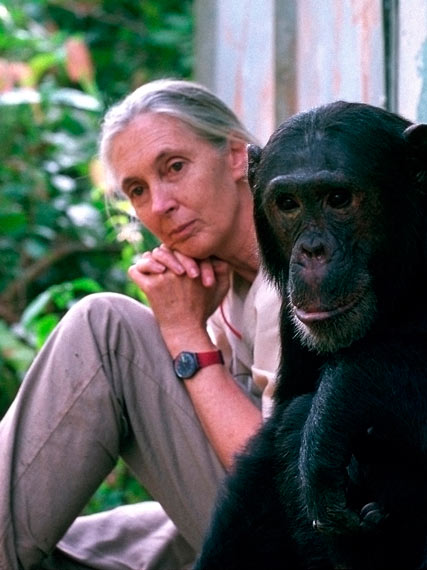
\includegraphics[scale=0.3]{jane_goodall.jpg}

    \uncover<2->{
      C'est \alert<3->{Jane Goodall}.
    }

    \uncover<3->{
      C'est \alert{elle}.
    }
  \end{frame}

  \begin{frame}{Qui est-ce? \gloss{Who is that?}}
    \centering
    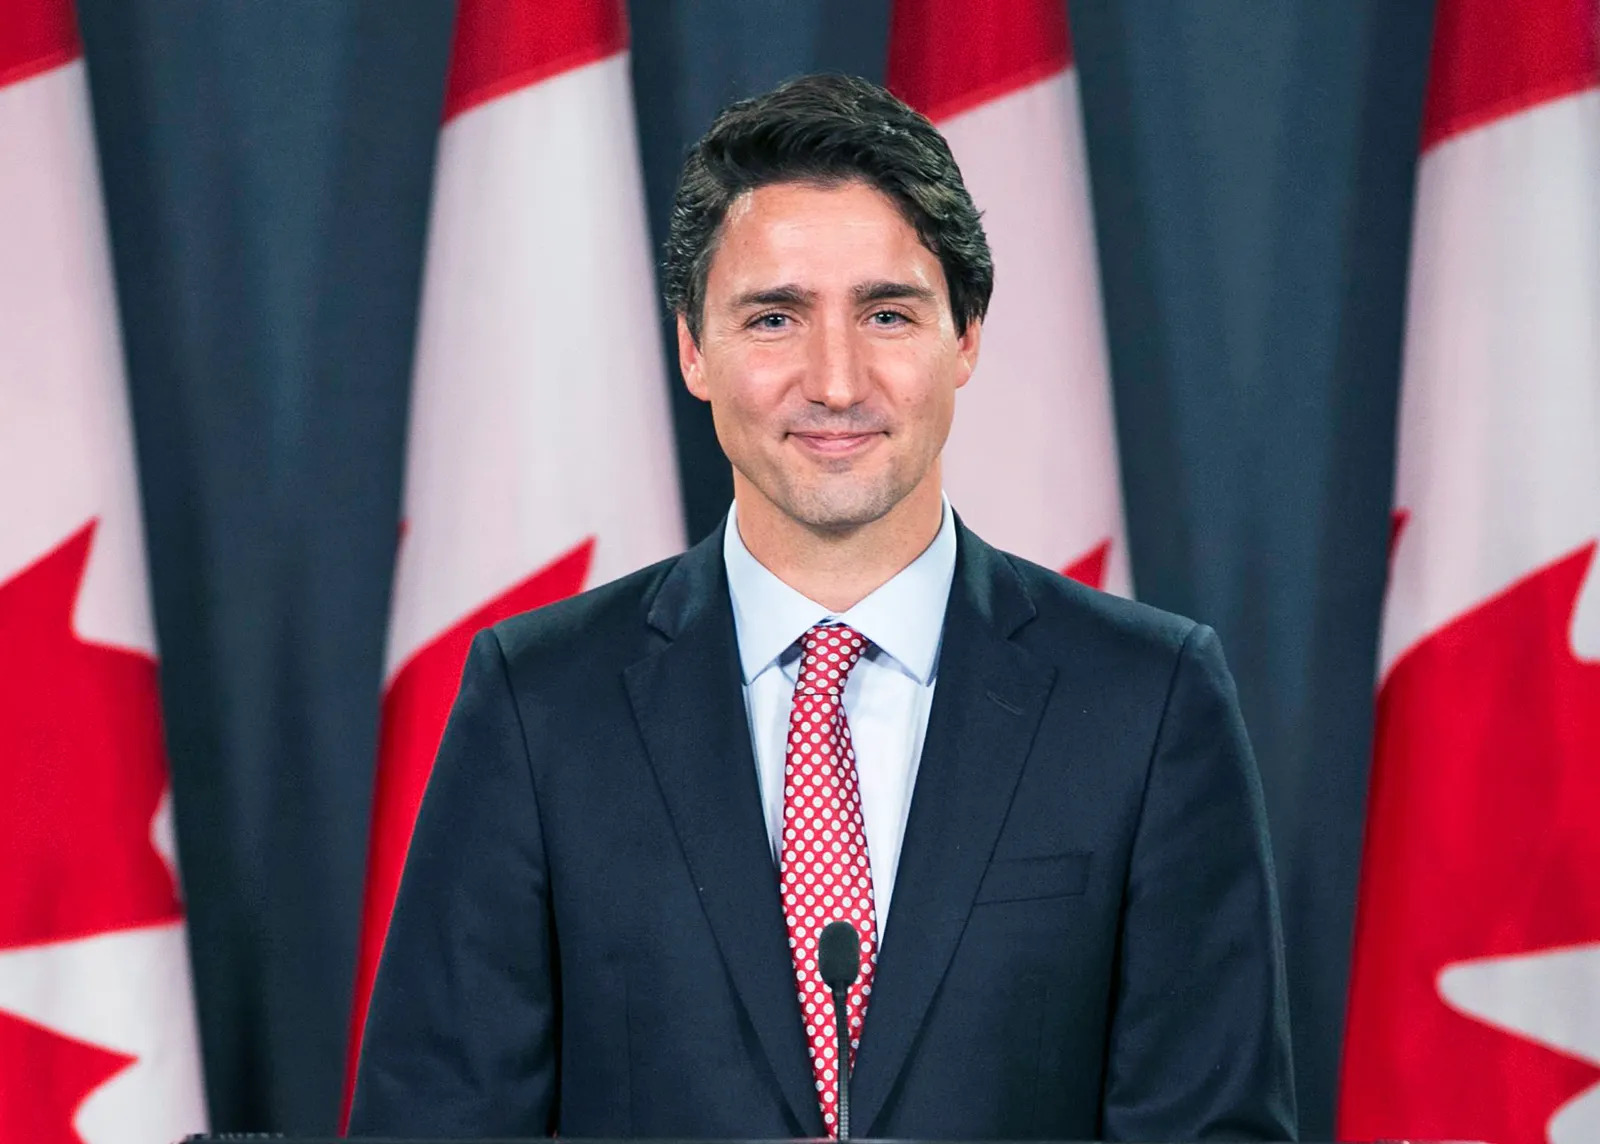
\includegraphics[scale=0.15]{trudeau.jpg}

    \uncover<2->{
      C'est \alert<3->{Justin Trudeau}.
    }

    \uncover<3->{
      C'est \alert{lui}.
    }
  \end{frame}

  \begin{frame}{Qui est-ce? \gloss{Who is that?}}
    \centering
    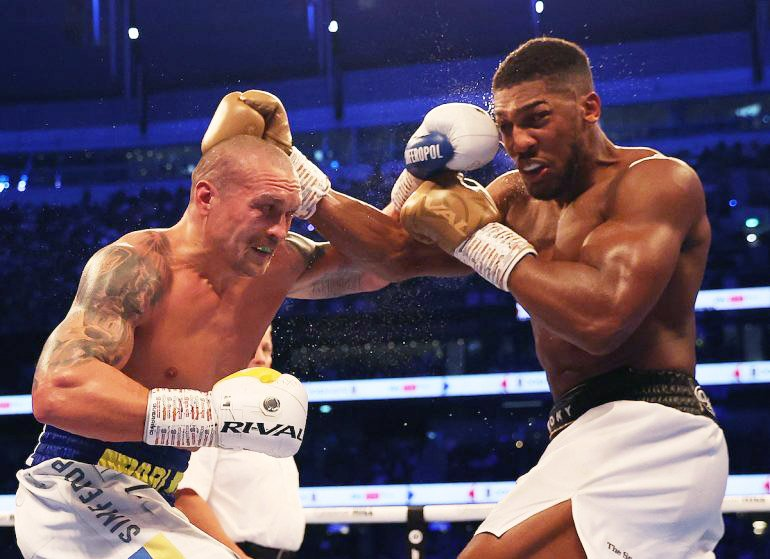
\includegraphics[scale=0.3]{usyk_joshua.jpg}

    \uncover<2->{
      Ce sont \alert<3->{Oleksandr Usyk et Anthony Joshua}.
    }

    \uncover<3->{
      Ce sont \alert{eux}.
    }
  \end{frame}

  \begin{frame}{Revue}
    \begin{columns}
      \column{0.5\textwidth}
        \begin{itemize}
          \item Salut!
          \item Comment tu t'appelles?
          \item toi $\to$ informel
        \end{itemize}
      \column{0.5\textwidth}
        \begin{itemize}
          \item Bonjour!
          \item Comment vous appelez-vous?
          \item vous $\to$ formel ou pluriel
        \end{itemize}
    \end{columns}
  \end{frame}

  \begin{frame}{Toi ou vous?}
    \gloss{Find a partner, and imagine that they are the person on their card.
    Introduce yourself, and ask each other how you are doing.
    For example:}

    \begin{columns}
      \column{0.46\textwidth}
        <E1 $\to$ teacher> \\
        <E2 $\to$ student>
        \begin{itemize}
          \item[E1:] Bonjour, je m'appelle Monsieur McNeill. Comment tu t'appelles?
          \item[E2:] Bonjour, je m'appelle ...
          \item[E1:] Comment ça va?
          \item[E2:] Je suis fatigué, et vous?
          \item[E1:] Je vais bien.
        \end{itemize}
      \column{0.54\textwidth}
        \begin{center}
          \begin{tabular}{| l l}
            ça va         & \gloss{fine} \\
            je vais bien  & \gloss{I'm fine} \\
            très bien     & \gloss{very well} \\
            pas mal       & \gloss{not bad} \\
            ça peut aller & \gloss{I'm getting by} \\
            ça va mal     & \gloss{things are going badly} \\
            en forme      & \gloss{in shape} \\
            fatigué       & \gloss{tired} \\
            malade        & \gloss{sick} \\
            occupé        & \gloss{busy} \\
            stressé       & \gloss{stressed out} \\
          \end{tabular}
        \end{center}
    \end{columns}
  \end{frame}

  \begin{frame}{}
    Questions?
  \end{frame}
\end{document}
